\documentclass{article}
\usepackage[utf8]{inputenc}
\usepackage{graphicx}
\usepackage{subcaption}
\usepackage{booktabs}
\usepackage{xcolor}

\begin{document}

\section{Non-IID Resilience Evaluation}

To evaluate resilience against statistical heterogeneity, we conduct experiments on FMNIST and CIFAR-10 using Dirichlet concentration parameters $\alpha \in \{0.1, 0.5, 1, 5, 10\}$.
As shown in Fig.~\ref{NoneIID_compare}, all methods exhibit higher test accuracy when $\alpha$ increases, since larger $\alpha$ produces more homogeneous client data distributions and thus eases global aggregation.

\begin{figure}[htbp]
    \centering
    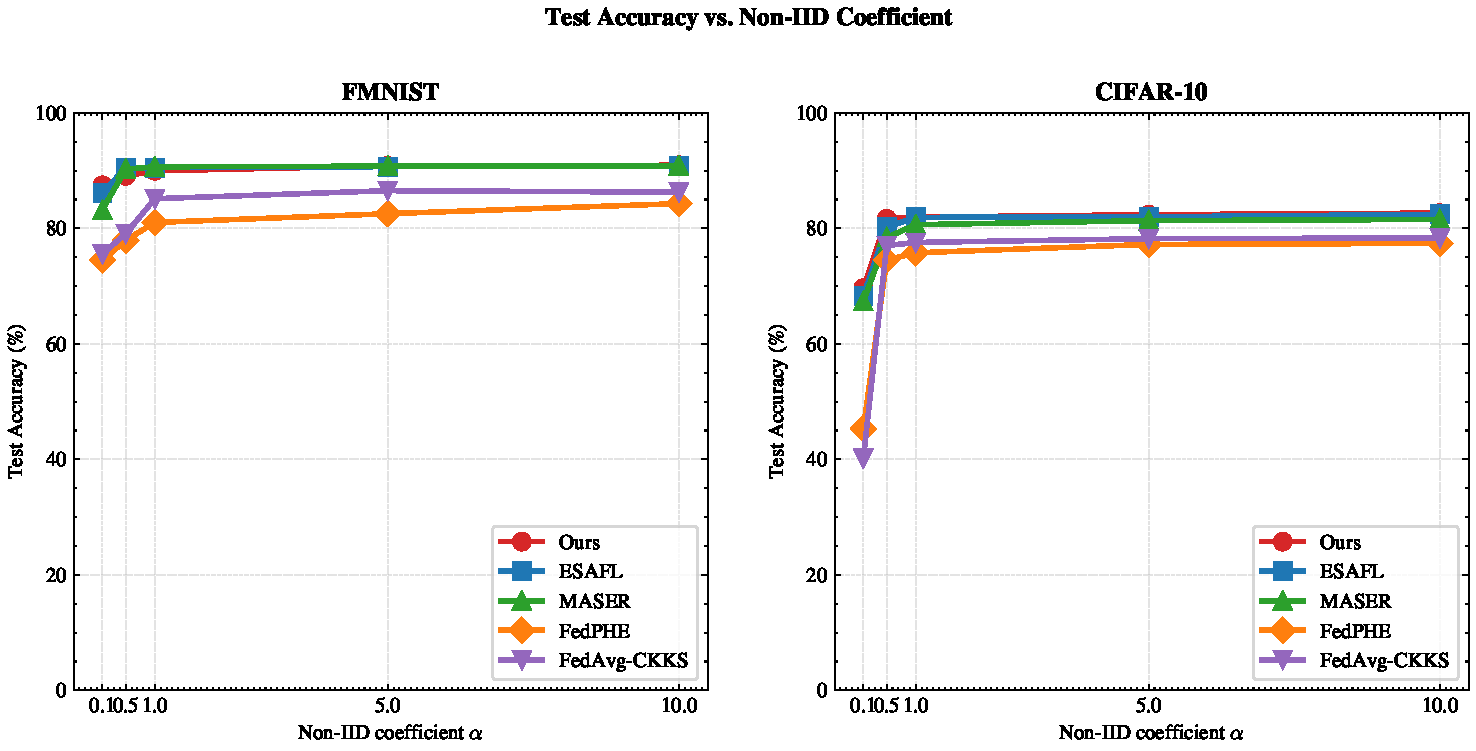
\includegraphics[width=0.95\textwidth]{pic/01_line_markers.pdf}
    \caption{Test accuracy of all compared methods under varying Non-IID coefficients on FMNIST (left) and CIFAR-10 (right).}
    \label{NoneIID_compare}
\end{figure}

\subsection{Observations on FMNIST}

On FMNIST, the top-performing methods are ESAFL and Ours, whose average accuracies reach $89.75\%$ and $89.65\%$, respectively, while MASER follows closely at $89.16\%$.
Moreover, at the most heterogeneous setting ($\alpha=0.1$), Ours achieves $87.45\%$, which is $1.28$ percentage points higher than ESAFL ($86.17\%$) and $4.22$ percentage points higher than MASER ($83.23\%$).
Consequently, the robustness ranking under severe heterogeneity is Ours $>$ ESAFL $>$ MASER.
In contrast, FedPHE and FedAvg-CKKS obtain only $74.50\%$ and $75.65\%$ at $\alpha=0.1$, respectively, although their accuracy improves considerably to $84.29\%$ and $86.27\%$ at $\alpha=10$.
Therefore, the gap between the encrypted-FL baselines and our method narrows as the data becomes more IID, yet it remains significant under strong heterogeneity.

\subsection{Observations on CIFAR-10}

On CIFAR-10, the overall trends are consistent with FMNIST, but the absolute accuracy drop under small $\alpha$ is much larger because CIFAR-10 is a more complex dataset.
Specifically, Ours attains $69.67\%$ at $\alpha=0.1$, whereas ESAFL and MASER achieve $68.31\%$ and $67.32\%$, respectively.
Furthermore, FedPHE and FedAvg-CKKS drop to $45.32\%$ and $40.21\%$, respectively, at $\alpha=0.1$, which indicates that standard encrypted aggregation is more vulnerable to severe client drift on difficult vision tasks.
Nevertheless, all methods recover substantially when $\alpha$ increases: for instance, FedAvg-CKKS rises by $38.13$ percentage points from $\alpha=0.1$ to $\alpha=10$.
As a result, at $\alpha=10$, the best methods converge to around $82\%$, and the relative differences become smaller.

\subsection{Summary}

In summary, Ours consistently yields the highest or near-highest accuracy under strong Non-IID settings on both datasets, while ESAFL and MASER remain competitive alternatives.
On the other hand, FedPHE and FedAvg-CKKS suffer larger accuracy degradation when $\alpha$ is small, primarily because they lack effective mechanisms to compensate for sparse or heterogeneous client updates.
Thus, the proposed ESP components---local sparsification, residual feedback, decay-based residual tracking, and ranking-based aggregation---jointly improve the model's robustness against statistical heterogeneity.

\end{document}
